\documentclass[../../main.tex]{subfiles}

\begin{document}

\section{Experimento 1: 45 períodos observados, 20 de dependencia} \label{sec:exp1}
En este primer escenario, tomamos 45 períodos observados previos al inicio del programa
para cada individuo con 20 períodos de dependencia, en donde permitimos un máximo de 6
incrementos. Así, la proporción de períodos de dependencia sobre períodos observados es de
0.44, y de subidas sobre períodos de dependencia de 0.3. Al tener 45 períodos observados
pre-tratamiento y 3 cohortes, los inicios de programa son 46, 47 y 48. Además, el valor
de \(\mu_{{EF}_{NiNi}}\) en este caso fue el mismo que para tratados y controles (10).

Consideramos que este escenario es el que más favorece a las redes ya que es en el que
mayor cantidad de períodos observados y de dependencia hay, por lo que lo tomamos como
punto de referencia para comparar lo ocurrido en los otros. Asimismo, creemos que tomar 45
períodos como la cantidad máxima en todos los escenarios es acorde con la realidad, en
donde en algunas situaciones puede resultar complicado tener información sobre más
períodos, como suele ocurrir, por ejemplo, en el caso de pequeñas y medianas empresas.

La Figura \ref{fig:time_series_exp1} muestra algunos ejemplos de las series de tiempo
generadas para cada uno de los grupos, en donde se ve claramente la tendencia que estamos
tratando de capturar en tratados y controles. En ellos, en los últimos 20 de los 45
períodos considerados se observa el comportamiento ``decreciente con ruido'', que en los
NiNi no está presente.

\begin{figure}[ht]
    \centering
    \begin{minipage}{0.48\textwidth}
        \centering
        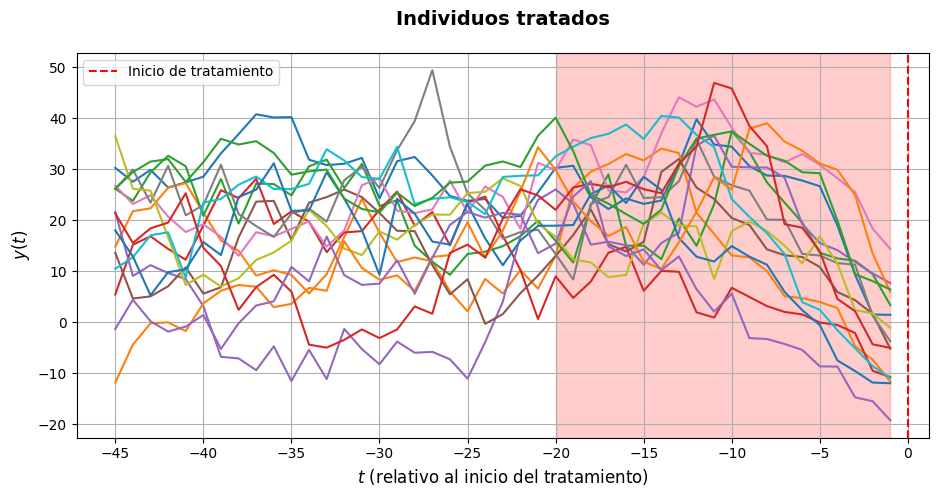
\includegraphics[scale=0.3]{figs/Exp1/tratados_sim61.png}
    \end{minipage}
    \hfill
    \begin{minipage}{0.48\textwidth}
        \centering
        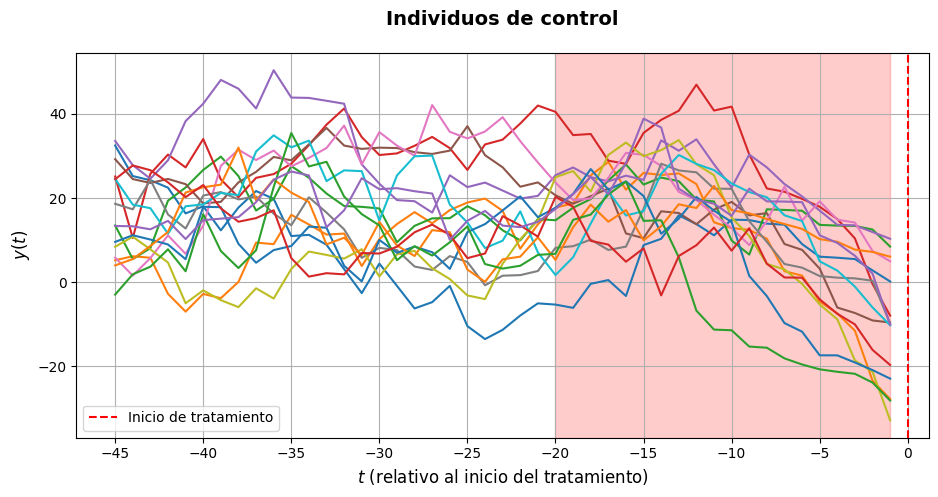
\includegraphics[scale=0.3]{figs/Exp1/controles_sim61.png}
    \end{minipage}
    \vspace{0.5em}
    \begin{minipage}{0.6\textwidth}
        \centering
        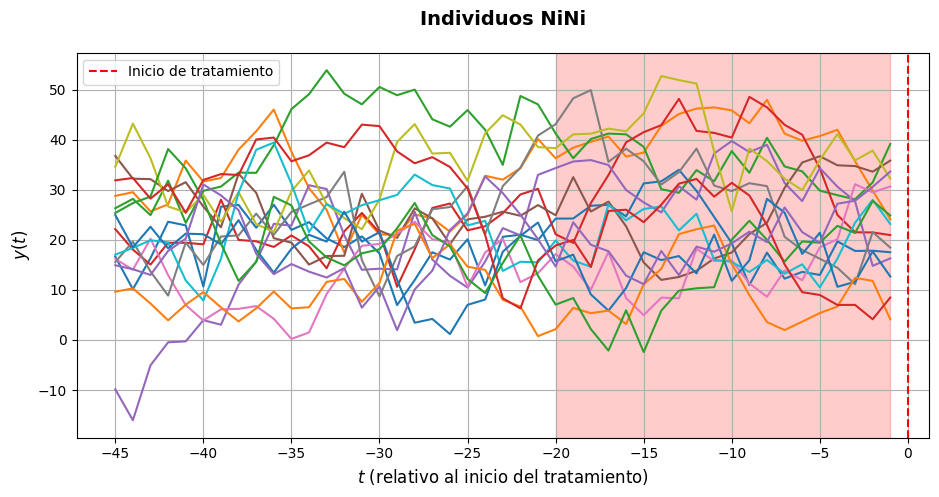
\includegraphics[scale=0.3]{figs/Exp1/ninis_sim61.png}
    \end{minipage}
    \caption{Ejemplos de series de tiempo generadas para cada grupo en el Experimento 1.
    Los períodos con un fondo rojo indican los períodos de dependencia para tratados y
    controles, en donde se modela la tendencia ``decreciente con ruido''. La línea
    punteada roja indica el inicio de tratamiento para cada individuo.}
    \label{fig:time_series_exp1}
\end{figure}


La Tabla \ref{tab:results_exp1} muestra los resultados obtenidos en las métricas \(F_1\),
precisión y cobertura por las diferentes redes y el PSM. Cada valor representa el
promedio de esa métrica en las 100 simulaciones en el conjunto de test, junto con la
desviación estándar.

\begin{table}[H]
    \centering
    \renewcommand{\arraystretch}{1.2}
    \begin{tabular}{|c|c|c|c|}
        \hline
        & \textbf{Puntaje} \(F_1\) & \textbf{Precisión} & \textbf{Cobertura} \\ \hline\hline
        \textbf{LSTM}
            & $0.80984 \pm 0.02679$ & $0.72408 \pm 0.04763$ & $0.92219 \pm 0.01823$ \\ \hline
        \textbf{Convolucional}
            & $\mathbf{0.83945 \pm 0.01999}$ & $\mathbf{0.76293 \pm 0.03537}$ & $\mathbf{0.93468 \pm 0.01383}$ \\ \hline
        \makecell{\textbf{LSTM +}\\\textbf{Convolucional}}
            & $0.83694 \pm 0.01836$ & $0.76084 \pm 0.03397$ & $0.93161 \pm 0.01418$ \\ \hline
        \textbf{PSM}
            & $0.65882 \pm 0.01561$ & $0.65998 \pm 0.01556$ & $0.65767 \pm 0.01573$ \\
        \hline
    \end{tabular}

    \caption{Promedios y desviaciones estándar de las métricas \(F_1\), precisión y
    cobertura sobre la clase positiva (controles), evaluadas en el conjunto de test en las
    100 simulaciones del Experimento 1 con las diferentes arquitecturas de redes
    neuronales y el PSM.}
    \label{tab:results_exp1}
\end{table}

En primer lugar, se puede ver que el desempeño de todas las redes fue superior al del PSM,
y consideramos que los resultados obtenidos con ellas son satisfactorios. En segundo
lugar, el rendimiento de las redes fue parecido entre ellas; más aún entre la
Convolucional y la LSTM + Convolucional, siendo la primera apenas mejor. Algo que también
se puede observar es que la cobertura obtenida con todas las redes es bastante alta, lo
cual indica que la mayoría de los controles fueron identificados por la red; mientras que
la precisión fue consistentemente menor, aunque con valores aceptables.

La Tabla \ref{tab:hyperparams_exp1} muestra, para cada arquitectura, el valor de cada
hiperparámetro que fue seleccionado con mayor frecuencia como el óptimo durante la
búsqueda en las 100 simulaciones. Consideramos que de utilizar alguna de las
arquitecturas, estos valores deberían ser los empleados para entrenarla.

\begin{table}[H]
    \centering
    \renewcommand{\arraystretch}{1.2}
    \begin{tabular}{|c|c|c|c|c|}
        \hline
            & \makecell{\textbf{Tamaño}\\\textbf{de lote}}
            & \makecell{\textbf{Neuronas en}\\\textbf{capas ocultas}}
            & \makecell{\textbf{Tasa de}\\\textbf{aprendizaje}}
            & \textbf{Dropout} \\ \hline\hline
        \textbf{LSTM}
            & 128 (44\%) & 128 (69\%) & 0.001 (98\%) & 0.3 (54\%) \\ \hline
        \textbf{Convolucional}
            & 32 (46\%)  & -          & 0.001 (90\%) & 0.3 (66\%) \\ \hline
        \makecell{\textbf{LSTM +}\\\textbf{Convolucional}}
            & 32 (37\%)  & 64 (37\%)  & 0.001 (86\%) & 0.3 (72\%) \\
        \hline
    \end{tabular}
    \caption{Valores de hiperparámetros seleccionados con mayor frecuencia en las 100
    simulaciones en cada arquitectura en el Experimento 1. Cada celda contiene dicho valor
    y entre paréntesis el porcentaje de simulaciones en el que resultó ser el mejor, de
    acuerdo a la optimización realizada por Optuna mediante validación cruzada.}
    \label{tab:hyperparams_exp1}
\end{table}

Se puede observar a simple vista que para todas las arquitecturas, la tasa de aprendizaje
de 0.001 resultó ser ampliamente la mejor y que en la mayoría de los casos se tomó un
dropout de 0.3, que era el menor en el espacio de búsqueda establecido. Otro detalle es
que el tamaño de lote parece no haber sido tan relevante, ya que en cada modelo, el valor
más seleccionado lo fue en menos de la mitad de las simulaciones. Algo que resulta
interesante es que en la LSTM ``sola'', el número de neuronas por capa más elegido fue
128, el máximo en el espacio de búsqueda, mientras que cuando se la combinó con la
Convolucional, este número se redujo a la mitad.

\end{document}